\section*{\fs{12}Zapytanie z podzapytaniem w From}
\par{
\fs{12}
\subsection*{\fs{12} Średnia ilość wizyt w ciągu roku}

\listsinglespacing{
\fs{12}
\begin{lstlisting}[frame=single,language=SQL,]
Select WW.ROK,AVG(WW.Ilosc) as [Średnia Roczna]
from (
		Select MONTH(W.data) as Ilosc,YEAR(W.data)  as Rok
		from Wizyty as W
		group by YEAR(W.data), MONTH(W.data)
		)
		as WW
group by WW.Rok

\end{lstlisting}
\begin{figure}[h!]
    \centering
   \scalebox{.85}{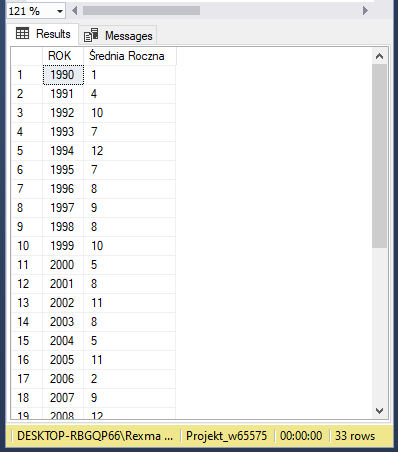
\includegraphics{Images/Zadanie3/P5/Z21a.png}}
    \caption{Wynik Zapytania}
    \label{fig:my_label}
\end{figure}
\begin{figure}[h!]
    \centering
   \scalebox{.60}{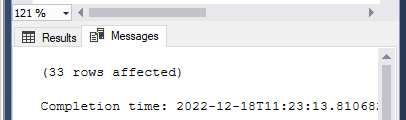
\includegraphics{Images/Zadanie3/P5/Z21b.png}}
    \caption{Wynik Zapytania}
    \label{fig:my_label}
\end{figure}
}
\newpage
\clearpage

\subsection*{\fs{12} Ilość wyjazdów na przestrzeni lat}

\listsinglespacing{
\fs{12}
\begin{lstlisting}[frame=single,language=SQL,]
Select Count(W.Miesiac) as Wyjazdy, W.Rok
From (
		Select Month(data_wyjazdu) as Miesiac,YEAR(data_wyjazdu) as Rok
		from Wyjazdy
		) as W
Group by W.Rok
\end{lstlisting}
\begin{figure}[h!]
    \centering
   \scalebox{.85}{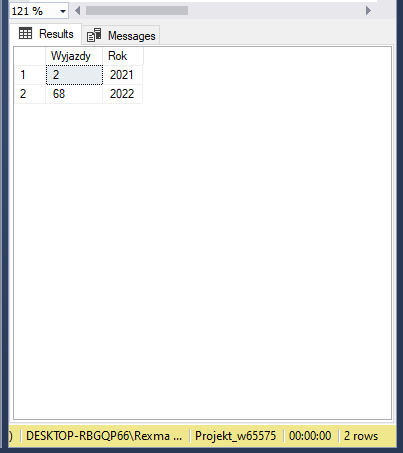
\includegraphics{Images/Zadanie3/P5/Z22a.png}}
    \caption{Wynik Zapytania}
    \label{fig:my_label}
\end{figure}
\begin{figure}[h!]
    \centering
   \scalebox{.60}{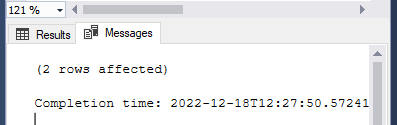
\includegraphics{Images/Zadanie3/P5/Z22b.png}}
    \caption{Wynik Zapytania}
    \label{fig:my_label}
\end{figure}
}
\newpage
\clearpage
\subsection*{\fs{12}Ilość wizyt w poszczególnych miesiącach w roku 2004 }


\listsinglespacing{
\fs{12}
\begin{lstlisting}[frame=single,language=SQL,]
Select Count(W.Dzien) as Ilosc, DATENAME( MONTH, DATEADD( MONTH, W.Miesiac, -1)) 
as Miesiac
From (
		Select Day(data) as Dzien,Month(data) as Miesiac,YEAR(data) as Rok
		from Wizyty 
		where YEAR(data)=2004
		) as W
Group by W.Miesiac

\end{lstlisting}
\begin{figure}[h!]
    \centering
   \scalebox{.85}{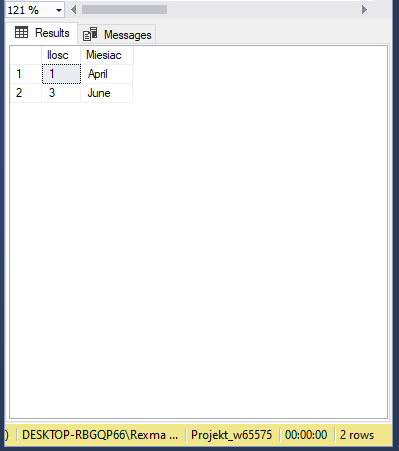
\includegraphics{Images/Zadanie3/P5/Z23a.png}}
    \caption{Wynik Zapytania}
    \label{fig:my_label}
\end{figure}

}

\begin{figure}[h!]
    \centering
   \scalebox{.60}{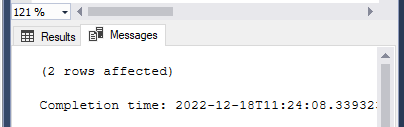
\includegraphics{Images/Zadanie3/P5/Z23b.png}}
    \caption{Wynik Zapytania}
    \label{fig:my_label}
\end{figure}



\newpage